\documentclass[13pt, a4paper, twoside]{article}
\usepackage[utf8]{inputenc}
\usepackage{geometry}
\usepackage[czech]{babel}
\usepackage{chemformula}
\usepackage{chemfig}
\usepackage{float}
\usepackage{caption}
\usepackage{enumitem}
\usepackage{fancyhdr}
\usepackage{setspace}
\usepackage{multicol}
\geometry{legalpaper, margin=1.05in}
\pagestyle{fancy}
\lhead{\Large Šárka Doležalová, skupina 6}
\rhead{\large 10.12.2020}
\begin{document}
    \begin{center}
        \Huge
        Úloha 2: Izolace glycinu a identifikace neznámé aminokyseliny
    \end{center}
    \large \onehalfspacing
    \section*{Zadané úlohy}
        \begin{enumerate}
            \item Z hydrochloridu glycinu izolujte pomocí chromatografie na iontoměniči
            volný glycin ve formě zwitteriontu
            \item Pomocí srovnávací tenkovrstevné chromatografie (TLC) identifikujte
            předložený vzorek aminokyseliny
        \end{enumerate}
    \section*{Teoretický úvod}
    \subsection*{Práce s rotační vakuovou odparkou}
    Slouží k rychlému odpaření většího množství rozpouštědla a získání látky v něm rozpuštěné.
    Baňka se kontinuálně otáčí a tím se na její povrchu obnovuje vrstvička roztoku, tu za
    pomoci vakua odpařujeme. Vakuum vytváříme membránovou pumpou a musíme dbát na to,
    aby směs neměla moc vysokou teplotu a nebo aby nevykypěla.

    \subsection*{Srážení přídavkem špatného rozpouštědla}
    Krystalizace založená na principu změny rozpouštědla. K roztoku s rozpouštědlem ve
    kterém se látka dobře rozpouští dodáme rozpouštědlo, ve kterém ale daná látka rozpustná
    není, jako výsledek dojde vyloučení látky v pevné fázi.

    \subsection*{Odsávání na fritě}
    Proces oddělení pevné fáze od kapalné za sníženého tlaku. Kapalnou fázi jímáme do
    odsávací baňky a pevná zůstáva na fritě, ke snížení tlaku se obyvykle používá vakuová
    pumpa nebo vývěva. 
    
    \subsection*{Chromatografie na ionexu}
    Ionexy neboli iontoměničové pryskyřice se používají k rozdělení iontových látek. Jsou to
    kopolymery inertního monomerů s monomerními jednotkami. Ty mají polární substituenty:
    kyselé nebo bazické. Ionexy jsou nejčastěji vloženy jako náplně ve sloupcových kolonách.
    Iontoměniče rozdělujeme na kationtové a aniontové. Po jejich používání je vždy potřeba
    udělat tzv. regeneraci.

    \subsection*{Dělení látek na chromatografické destičce}
    Princip TLC analýzi je založen na chromatografické destičce se silikagelem jejichž povrch je
    silně polární a tím pádem má vysokou afinitu k polárním sloučeninám zejména aminům. Při
    použití jako mobilní fáze amoniaku bude platit, že čím větší polarita sloučeniny, tím méně se
    bude pohybovat
    K následné vizualizace aminokyselin se používá ninhydrin, který obarvuje aminokyseliny na
    fialovo

    \section*{Postup}
    \subsection*{Izolace glycinu}
    Iontoměnič byl převeden do kyselého cyklu, přidáním 25 ml zředěné HCl a jejím protékáním
    rychlostí 1 kapka za 1 sekundu. Poté byl promyt iontoměnič destilovanou vodou do
    neutrality. Bylo naváženo 1,00 g hydrochloridu glycinu. Hydrochlorid glycinu byl potom
    rozpuštěn v malém množství vody. Roztok byl pomocí kapátka nanesen na sloupec ionexu.
    Sloupec ionexu byl opět promyt destilovanou vodou do neutrality. Po nastolení neutrality byl
    glycin jímán do baňky o objemu 250 ml. Pro eluci glycinu bylo použito 100 ml 5% roztoku
    amoniak vu. Amoniak byl přidáván po malých dávkách a kolonou protékal pomalou rychlostí.
    Následně byl sloupec opět převeden do kyselého cyklu. Frakce amoniaku byla odpařena za
    použití odparky. Po vymytí amoniaku byla dále kolona regenerována za použití 10% HCl a
    potom opět promyta do neutrality. Odpařený glycin byl rozpuštěn v malém množství vody a
    roztok byl znovu odpařen do sucha. PO opětovném odpaření byl glycin zase rozpuštěn v
    malém množství vody. Do kádinky bylo odměřeno 80 ml acetonu a vodný roztok glycinu byl
    přidán pomocí kapátka, tím byl glycin vystrážen. Vysrážený glycin byl odsát na fritě. Produkt
    byl převeden na hodinové sklo a zvážen (m=0,5 g)

    \subsection*{Identifikace neznámé kyseliny}
    Na TLC destičku byly naneseny jednotlivé standardy aminokyselin (glycin, valin, fenylalanin
    a lysin) a neznámý vzorek. Při nanášení jsme opatrní, abychom jednotlivé látky nezanesly.
    Po zaschnutí vzorků byla TLC destička vyvíjena ve vyvíjecí cele, na jejím dně byla vrstvička
    mobilní fáze. Po vyvíjení byla destička vyjmuta a bylo označeno, kam až mobilní fáze došla
    tzv. čelo. Horkovzdušnou pistolí mobilní fáze byla vysušena. Následně byla provedena
    detekce skvrn. Na destičku byl rozprášen roztok ninhydrinu a poté byla opět zahřívána.
    Porovnáváním skvrn byl identifikován náš vzorek.
    
    \section*{Výpočty}
        \begin{align*}
            m_{hydrochlorid\: glycin}&=1.00\: g \:|\: M_{hydrochlorid\: glycin}=111.5\: g\cdot m^{-1}\\
            m_{glycin}&=0.50\: g\:| \: M_{glycin}=75.07\: g\cdot m^{-1}
        \end{align*}


        \begin{align*}
            n&=\frac{m_{hydrochlorid\: glycin}}{M_{hydrochlorid\: glycin}}\\
            \to \alpha&=\frac{m_{glycin}}{n \cdot M_{glycin}}\\
            \alpha&=73.6\%
        \end{align*}

    \subsection*{Retenční faktory}
    \begin{figure}[H]
        \centering
        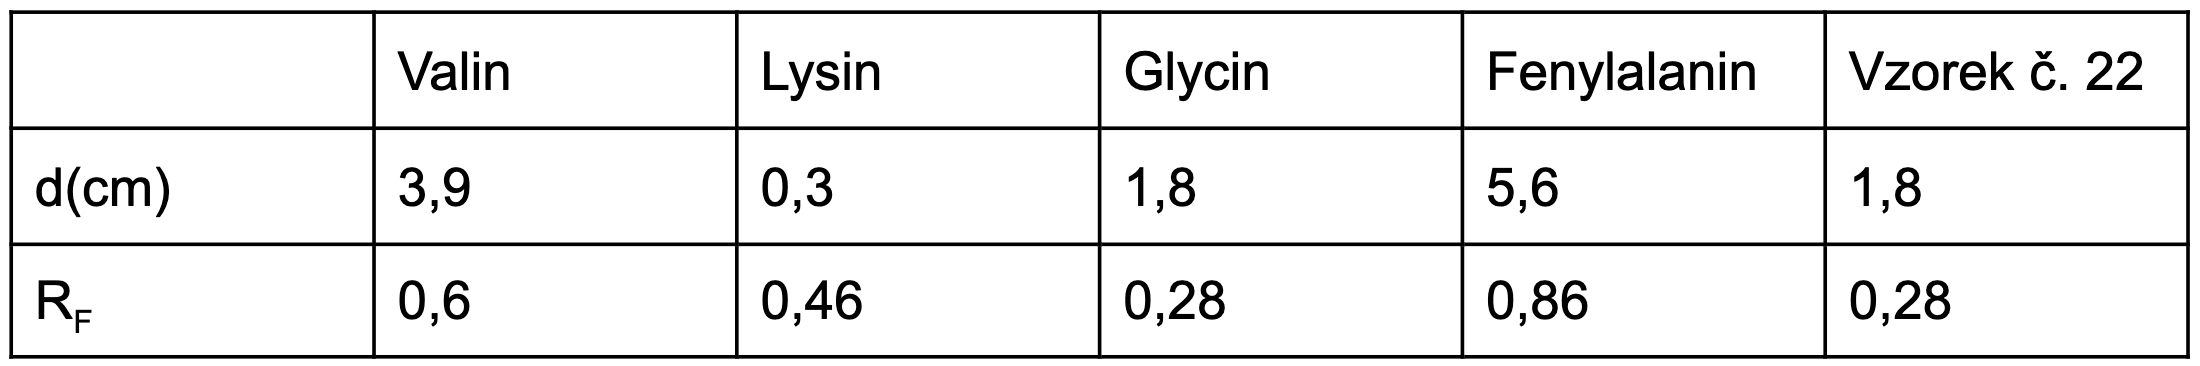
\includegraphics[width=6.5in]{uloha_2_tab_1.png}
        \caption*{Tab. 1: Retenční faktory}
    \end{figure}
    \section*{Závěr}
    Výtěžek čistého glycinu z 1,00 g hydrochloridu glycinu byl 73,6\%.
    Porovnáním skvrn jednotlivých aminokyselin bylo zjištěno, že neznámý vzorek č. 22 byl
    glycin.
    
\end{document}